% HW1 for Intro to Data Science
% also my first real foray into LaTeX ._.

\documentclass{article} 
\usepackage{fancyhdr, titling, graphicx, mathtools, fixltx2e, tikz}
\pagestyle{fancy}
\usetikzlibrary{positioning}
\newdimen\nodeDist
\nodeDist=35mm

% put name and page number in header
\fancyhead[L]{Green, Ben}
\fancyhead[R]{Page \thepage}

\author{Ben Green}
\title{Intro to Data Science HW 2}

\begin{document}

% title page
\begin{titlepage}
	\begin{center}
	\textsc{\LARGE Intro to Data Science HW 2}\\
	\vspace{3mm}
	
	{\large \theauthor}\\
	
	\tableofcontents
	\setcounter{secnumdepth}{0}
	\vfill
	
	{\large \today}
	\end{center}

\end{titlepage}

\section{Question 1}

\subsection{1a.}

The probability of a bit in the array remaining 0 is:

\begin{equation}
e^\frac{-20}{99}
\end{equation}

\noindent which comes out to .819. So, 1-.819 = .181 is the expected fraction of 1's.

\subsection{1b.}

The expected fraction of 0's is 1-.181 = .819

\section{Question 2}

The false positive rate is:

\begin{equation}
(1-e^{\frac{-3*2}{11}}) = (1-e^\frac{-6}{11})
\end{equation}

\section{Question 3}

\begin{center}
\begin{table}[h]
\begin{tabular}{|l|l|l|l|l|l|l|l|l|l|}
\hline
\textbf{a} & \textbf{b} & \textbf{c} & \textbf{a} & \textbf{d} & \textbf{e} & \textbf{a} & \textbf{c} & \textbf{b} & \textbf{b} \\ \hline
1          &            &            &            &            &            &            &            &            &            \\ \hline
.9         & 1          &            &            &            &            &            &            &            &            \\ \hline
.81        & .9         & 1          &            &            &            &            &            &            &            \\ \hline
           & .81        & .9         & 1.81       &            &            &            &            &            &            \\ \hline
           & .729       & .81        & 1.1629     & 1          &            &            &            &            &            \\ \hline
           & .6561      & .729       & 1.4661     & .9         & 1          &            &            &            &            \\ \hline
           & .5905      & .6561      &            & .81        & .9         & 2.4661     &            &            &            \\ \hline
           & .5314      &            &            & .729       & .81        & 2.219      & 1.6561     &            &            \\ \hline
           &            &            &            & .6561      & .729       & 1.997      & 1.4904     & 1.5314     &            \\ \hline
           &            &            &            & .5905      & .6561      & 1.797      & 1.3413     &            & 2.5314     \\ \hline
\end{tabular}
\end{table}
\end{center}

\section{Question 4}

(3x +7) mod 11\\
X=1, 10 mod 11 = 10, 1010\\
x=2, 13 mod 11 = 2, 0010\\
X=3, 16 mod 11 = 5, 0101\\
X=4, 19 mod 11 = 8, 1000\\
X=5, 22 mod 11 = 0, 0000\\
X=6, 25 mod 11 = 3, 0011\\
X=7, 28 mod 11 = 6, 0110\\
X=8, 31 mod 11 = 9, 1001\\
X=9, 34 mod 11 = 1, 0001\\
X=10, 37 mod 11 = 4, 0100\\

\noindent Set \{10 9 1 7\} would have to be in the set since the estimate of the number of distinct elements is 2\textasciicircum r where r is the max tail length in the set.

\section{Question 5}

\begin{center}

\begin{tikzpicture}[
    node/.style={%
      draw,
      rectangle,
    },
  ]

    \node [node] (A) {A};
    \path (A) ++(-135:\nodeDist) node [node] (B) {yes};
    \path (A) ++(-45:\nodeDist) node [node] (C) {B};
    \path (C) ++(-135:\nodeDist) node [node] (D) {C};
    \path (C) ++(-45:\nodeDist) node [node] (E) {no};
    \path (D) ++(-135:\nodeDist) node [node] (F) {yes};
    \path (D) ++(-45:\nodeDist) node [node] (G) {no};

    \draw (A) -- (B) node [left,pos=0.25] {true}(A);
    \draw (A) -- (C) node [right,pos=0.25] {false}(A);
    \draw (C) -- (D) node [left,pos=0.25] {true}(A);
    \draw (C) -- (E) node [right,pos=0.25] {false}(A);
    \draw (D) -- (F) node [left,pos=0.25] {true}(A);
    \draw (D) -- (G) node [right,pos=0.25] {false}(A);
\end{tikzpicture}
\end{center}

\section{Question 6}

\subsection{6a.}
\begin{equation}
H[12+,9-] = -\frac{12}{21}log_{2}\frac{12}{21} - \frac{9}{21}log_{2}\frac{9}{21} = -.5714 * -.8074 - .4286 * -1.2223 = .9852
\end{equation}

\subsection{6b.}
\begin{equation}
IG(X1) = T[7+, 1-] F[5+, 8-]
\end{equation}
\begin{equation}
.9582 - \frac{8}{21}*1.3925 - \frac{13}{21} * .6920 = .0265
\end{equation}
\begin{equation}
IG(X2) = T[7+, 3-] F[5+, 6-]
\end{equation}
\begin{equation}
.9852 - \frac{10}{21} * 1.0704 - \frac{11}{21} * 9329 = .013
\end{equation}

\subsection{6c.}

\begin{center}
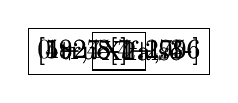
\begin{tikzpicture}[
    node/.style={%
      draw,
      rectangle,
    },
  ]

    \node [node] (A) {X1};
    \path (A) ++(-135:\nodeDist) node [node] (B) {0.924 [7+, 1-]};
    \path (A) ++(-45:\nodeDist) node [node] (C) {[5+, 8-] .1756};
    \path (C) ++(-45:\nodeDist) node [node] (E) {X2};
    \path (E) ++(-135:\nodeDist) node [node] (F) {.4827 [4+, 3-]};
    \path (E) ++(-45:\nodeDist) node [node] (G) {[1+, 5-] .2996};

    \draw (A) -- (B) node [left,pos=0.25] {true}(A);
    \draw (A) -- (C) node [right,pos=0.25] {false}(A);
    \draw (C) -- (E) node [right,pos=0.25] {}(A);
    \draw (E) -- (F) node [left,pos=0.25] {true}(A);
    \draw (E) -- (G) node [right,pos=0.25] {false}(A);
\end{tikzpicture}
\end{center}



\subsection{6d.}
\begin{equation}
\frac{4}{7} = .5714
\end{equation}
\section{Question 7}

Assuming that you've picked door number 1, there are three (equally likely) possible scenarios:

\begin{enumerate}
\item You pick the door with the prize, and the other two doors are empty.
\item Both your door and door number 2 are empty.
\item Both your door and door number 3 are empty.
\end{enumerate}

Overall, there are two groups of possibilities - that you've picked a winning door (1/3) or you've picked an empty door (2/3).\\

If an empty door is revealed, it must either be door 2 or 3, because you picked door number 1. Now you are presented with the same two groups - but the second group's doors now have probabilities 0 and 2/3 of containing the prize, when originally they were 1/3 each.\\

Since your door (door number 1) has a probability of 1/3 and the other closed door has a probability of 2/3, you should switch doors.



\end{document}